\section{Reconhecimento Facial}

O reconhecimento facial é uma das atividades mais comuns realizadas diariamente por seres vivos dotados de certa inteligência. Essa simples atividade vem despertando o interesse de pesquisadores que trabalham com Visão Computacional e Inteligência Artificial. O objetivo desses pesquisadores é de construir sistemas artificiais capazes de realizar o reconhecimento de faces humanas e a partir desta capacidade construir os mais diferentes tipos de aplicações: sistemas de vigilância, controles de acesso, definções automáticas de perfis, entre outros \cite{oliveira}.

No anos 70, os estudos do reconhecimento facial eram baseados sobre atributos faciais mensuráveis como olhos, nariz, sobrancelhas, bocas, entre outros. Porém, os recursos computacionais eram escassos e os algoritmos de extração de características eram ineficiêntes. Nos anos 90, as pesquisas na área ressurgiram, inovando os métodos existentes \cite{hong, saocarlos} e disseminando a técnica.

Um dos motivos que incentivou os diversos estudos sobre reconhecimento facial são as vantagens que o mesmo possui em relação a impressão digital e a íris.  No reconhecimento por impressão digital, a desvantagem consiste no fato que nem todas as pessoas possuem uma impressão digital com ``qualidade'' suficiente para ser reconhecida por um sistema. Já o reconhecimento por íris apresenta uma alta confiabilidade e larga variação, sendo estável pela vida toda. Porém, a desvantagem está relacionada ao modo de captura da íris que necessita de um alinhamento entre a câmera e os olhos da pessoa \cite{saocarlos}. 

Basicamente existem duas particularidades que fazem da face uma característica biométrica bastante atrativa \cite{drovetto}:

	\begin{enumerate}
		\item A aquisição da face é feita de forma fácil e não-intrusiva;
		\item Possui uma baixa privacidade de informação: como a face é exposta constantemente, caso uma base de faces seja roubada, essas informações não representam algum risco e não possibilitam um uso impróprio;
	\end{enumerate}

Umas das maiores dificuldades dos sistemas de reconhecimento é tratar a complexidade dos padrões visuais. Mesmo sabendo que todas as faces possuem padrões reconhecidos, como boca, olhos e nariz, elas também possuem variações únicas que devem ser utilizadas para determinar as características relevantes. Outra dificuldade encontrada em relação a essas características é que elas possuem uma larga variação estatística para serem consideradas únicas para cada indivíduo. O ideal seria que a variância inter-classe seja grande e a intra-classe pequena, pois assim imagens de diferentes faces geram os códigos mais diferentes possíveis, enquanto imagens de uma mesma face geram os códigos mais similares possíveis. Portanto, estabelecer uma representação que capture as características ideias é um difícil problema \cite{saocarlos}.

Do ponto de vista geral, o recohecimento facial continua sendo um problema aberto por causa de várias dificuldades que aumentam a variância intra-classe \cite{hong}. Entre estas, destacamos as mais comuns \cite{saocarlos}:

	\begin{itemize}
		\item iluminação;
		\item ângulos e poses;
		\item expressões;
		\item comésticos e acessórios;
		\item extração da face do contexto ou do fundo;
	\end{itemize}

No contexto de identificação, o reconhecimento facial se resume no reconhecimento de um ``retrato'' frontal, estático e controlado. Estático pois os ``retratos'' utilizados nada mais são que imagens, podendo ser tanto de intensidade quanto de profunidade e controlado pois a iluminação, o fundo, a resolução dos dispositivos de aquisição e a distância entre eles e as faces são essencialmente fixas durante o processo de aquisição da imagem \cite{hong}.

Basicamente, o processo de reconhecimento facial pode ser divido em duas tarefas principais \cite{hong}:

	\begin{enumerate}
		\item Detecção de faces em imagens;
		\item Reconhecimento das faces encontradas;
	\end{enumerate}

Falaremos dessas duas tarefas separadamente nas próximas subseções.



\subsection{Detecção de Faces em imagens}
	
A primeira etapa para o reconhecimento de faces é a detecção de um rosto, e a partir daí a comparação do mesmo com modelos conhecidos pelo sistema \cite{hong, oliveira}. Em um sistema de reconhecimento facial, tanto o tempo de resposta quanto a confiabilidade desta etapa influência diretamente no desempenho e o emprego deste sistema \cite{oliveira}.

A detecção de faces é definida como o processo que determina a existência ou não de faces em uma imagem e uma vez encotrada alguma face, sua localização deve ser apontada através de um enquadramento ou através de suas coordenadas dentro da imagem \cite{oliveira}. A figura \ref{enquadramentoRosto} representa um exemplo da detecção de uma face em uma imagem.

	\begin{figure}[hbt]
		\begin{center}
			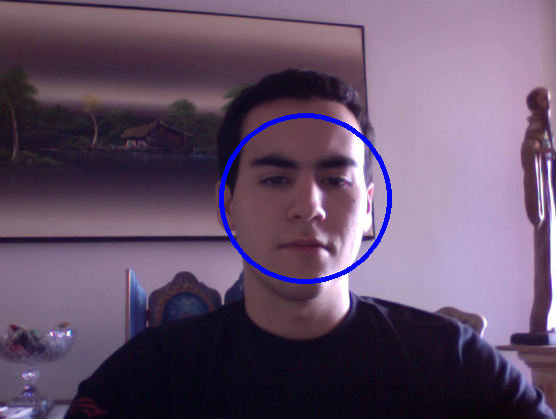
\includegraphics[height=9.5cm,width=12.5cm]{figuras/2.FundamentacaoTeorica/enquadramentoRosto.png}
		\end{center}
		\caption{Exemplo de um processo de detecção de uma face em uma imagem.}
		\label{enquadramentoRosto}
	\end{figure}

O processo de detecção de faces geralmente é pelas seguintes razões mostradas a seguir:

	\begin{enumerate}
		\item \textbf{Pose}: as imagens de uma face podem variar de acordo com a posição relativa entre a camêra e a face (frontal, 45 graus, perfil, ``de cabeça para baixo''), e com isso algumas características da face, como olhos e nariz, podem ficar parcialmente ou totalmente ocultadas \cite{yang}.
		\item \textbf{Presença de acessórios}: características faciais básicas importantes para o processo de detecção podem ficar ocultadas pela presença de acessórios, como óculos, bigode, barba, entre outros \cite{oliveira, yang}. 
		\item \textbf{Expressões faciais}: embora a maioria das faces apresente estruturas semelhantes (olhos, bocas, nariz, entre outros) e são dispostas aproximadamente na mesma configuração de espaço, pode haver um grande número de componentes não rigídos e texturas diferentes entre as faces. Um exemplo são as flexibilizações causadas pelas expressões faciais \cite{oliveira, yang};
		\item \textbf{Obstrução}: faces podem ser obstruídas por outros objetos. Em uma imagem com várias faces, uma face pode obstruir outra \cite{yang}.
		\item \textbf{Condiçoes da imagem}: a não previsibilidade das condições da imagem em ambientes sem restrições de ilimuniação, cores e objetos de fundo \cite{oliveira, yang}.
	\end{enumerate}

Atualmente, já existem diferentes métodos/técnicas de detecção de faces. Faleremos um pouco sobre os métodos baseados em imagens de itensidade e de cor e depois falaremos sobre os baseados em imagens 3D.


% Os métodos baseados em imagens de intensidade e cor podem ser divididos em 4 categorias \cite{yang}:

% 	\begin{enumerate}
% 		\item \textbf{``Knowladge-based methods'':} métodos, desenvolvidos principalmente para localização facial, beaseados em regras derivadas do conhecimento dos pesquisadores do que constitui uma típica face humana. Normalmente, captura as relações existentes entre as características faciais. É fácil econtrar regras que descrevem as caracterísicas faciais. Por exemplo, uma face sempre é constituída por dois olhos simétricos, um nariz e uma boca. As relações entre essas características podem ser representadas pelas distâncias relativas e posições.  \cite{yang};

% 		\item \textbf{``Feature invariant approaches'':} esses algoritmos tem como objetivo principal encontrar as características estruturais que existem mesmo quando a postura, ``ponto de vista'', condições de iluminação variam. E por meio dessas características localizar a face. São desenvolvidos principalmente para localização facial \cite{yang};

% 		\item \textbf{``Template matching methods'':} vários padrões comuns de um rosto são armazenados tanto para descrever o rosto como um todo quanto para descrever as características faciais separadamente. As correlações entre as imagens de entrada e os padrões armazenados são comuptados para detecção. Esses métodos são desenvolvidos para serem utlizados como localização e detecção facial \cite{yang};

% 		\item \textbf{``Appearence-based methods'':} Em contraste com os métodos do item anterior, os modelos são retirados de um conjunto de imagens de treinamento que devem capturar a variabilidade da face. Esses modelos retirados são utilizados para detecção. São métodos desenvolvidos principalmente para detecção de faces \cite{yang};

% 	\end{enumerate}

Um problema relacionado e muito importante é como avaliar a performance dos métodos de detecção de faces propostos. Com isso, muitas métricas foram adotadas como tempo de aprendizagem, número de amostras necessárias no treinamento e a proporção entre taxas de detecção e ``falso alarme''. Esta última é dificultada pelas diferentes definições para as taxas de detecção e falso alarme adotadas pelos pesquisadores \cite{yang}.

\subsection{Reconhecimento das Faces encontradas}

Na etapa de reconhecimento, as faces detectadas e processadas, serão comparadas com um banco de dados de faces conhecidas. Essa comparação tem uma acurácia media de 30-70\% entre as diversas técnicas. Esse é um forte campo de pesquisa desde a decada de 90 e as técnicas se invovam ano ápos ano.

	Técnicas 2D:
	\begin{enumerate}
		\item \textbf{Eigenfaces}
		\item \textbf{Redes Neurais}
		\item \textbf{Fisher Faces}
	\end{enumerate}

Reconhecimento facial 3D evita problemas comum em reconhecimentos faciais 2D como a mudança na iluminação, diferentes expressões faciais, maquiagem e orientação da cabeça.
	Técnicas 3D:
	\begin{enumerate}
		\item \textbf{``Face Recognition Homepage''}
		\item \textbf{``3D Face Recognition''}
		\item \textbf{``Active Appearance Models''}
	\end{enumerate}



Eigenface é um algoritmo de reconhecimento de face simples e fácil de implementar. Os passos utilizados pelo Eigenface também são utilizados em muitos métodos avançados. Os princípios básicos por trás dele como PCA(``Principal Component Analisys'') e ``distance-based matching'' aparecem mais e mais na computação visual e aplicações diversas de maquinas inteligentes.
O Eigenface trabalha de forma simples, dada uma imagem de um rosto desconhecido e imagens exemplos de pessoas conhecidas.
	\begin{enumerate}
		\item Computa a distância entre a nova imagem e cada uma das imagens já conhecidas.
		\item Seleciona a imagem mais proxima do novo rosto.
		\item Se a distância da nova imagem para a imagem exemplo for maior que o limite predefinido, ``reconhece'' a imagem caso contrario classifica como ``desconhecida''.
	\end{enumerate}


A distância entre as imagens é medida ponto a ponto. Esta é também chamado de distância euclidiana. Em duas dimensões (2D), a distância euclidiana entre os pontos $P_1$ e $P_2$ \ref{distanciaEntrePontos}.
 
 	\begin{equation}
 	d_{12} = \sqrt(d_{x2} + d_{y2}),  onde    d_x = x_2-x_1 e d_y = y_2-y_1.
 	\end{equation}

    \begin{figure}[hbt]
		\begin{center}
			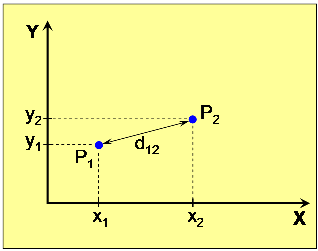
\includegraphics[height=9.5cm,width=12.5cm]{figuras/2.FundamentacaoTeorica/graficoDistanciaEntrePontos.png}
		\end{center}
		\caption{Distância Euclidiana entre dois pontos em duas dimensões.}
		\label{distanciaEntrePontos}
	\end{figure}


Imagens possuem ``ruídos'' e vamos definir ruído como qualquer coisa que atrapalhe na identificação, intensidade de luz é uma delas. Cada pixel possui uma intensidade de ruído diferente e com cada pixel dando a sua contribuição fica muito difícil encontrar a imagem correta. Uma solução é diminuir a dimensionalidade da imagem tornando assim o ruido menor e sendo possível extrair as informações importante da imagem.

Um dos metodos existentes para redução de imagem é o PCA - Principal Components Analysis.

Para se ter uma ideia do que é o PCA, vejamos um caso especial de PCA chamado de ``least squares line fit". O lado esquerdo da Figura \ref{exemploPCA} mostra um exemplo de uma linha de montagem em três pontos: os locais do mapa em 2D para Los Angeles, Chicago e Nova York.

Estes três pontos do mapa são quase, mas não completamente, em uma única linha já. Se você estava planejando uma viagem, essa relação já seria uma informação útil. Nesse sentido, uma única linha expressa algo essencial sobre seu relacionamento. A linha tem apenas uma dimensão, por isso, se podemos substituir localizações dos pontos de 2D com localizações ao longo de uma única linha, vamos ter reduzido a sua dimensionalidade.

Como eles já estão quase alinhados, uma linha pode ser traçada através deles com pouco erro. O erro no ajuste da linha é medido pela soma do quadrado da distância de cada ponto da linha. A linha de melhor ajuste é aquele que possui o menor erro.

	\begin{figure}[hbt]
		\begin{center}
			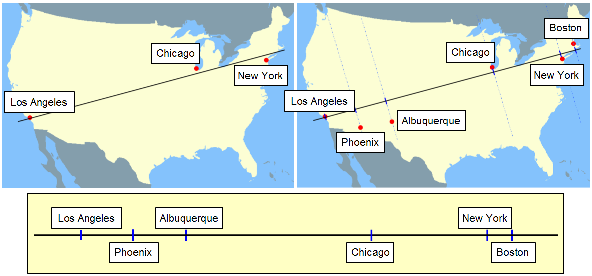
\includegraphics[height=9.5cm,width=12.5cm]{figuras/2.FundamentacaoTeorica/PCAexemploMapa.png}
		\end{center}
		\caption{Mapa}
		\label{exemploPCA}
	\end{figure}

Embora a linha encontrada acima é um objeto 1D, é localizado dentro de um espaço maior, 2D, e tem uma orientação, sua inclinação. A inclinação da linha expressa algo importante sobre os três pontos. Ele indica a direção em que eles estão espalhados mais.


Se posicionarmos a origem do nosso plano cartesiano em algum lugar dessa linha, podemos escrever a equação da linha como uma simples $y = mx$, onde m é a inclinação da linha: $dy / dx$.

Quando ele é descrito desta maneira, a linha é um subespaço do espaço 2D definido pelo sistema de coordenadas. Esta descrição enfatiza o aspecto dos dados que estamos interessados, ou seja, a direção que mantém esses pontos mais separados um do outro.

Esta direção da separação máxima é chamada de primeira componente principal de um conjunto de dados. A direção com a separação próxima maxima é a perpendicular a esta. Essa é a segunda componente principal. Em um conjunto de dados 2D, podemos ter no máximo dois componentes principais.

No entanto, o número de componentes principais, podemos encontrar também é limitada pelo número de pontos de dados. Para ver o porque disto podemos pensar em um conjunto de dados que consiste de apenas um ponto. Qual é o sentido da separação máxima para esse conjunto de dados? Não há um só, porque não há nada para separar. Agora, considere um conjunto de dados com apenas dois pontos. A linha que conecta esses dois pontos é o primeiro componente principal. Mas não há segundo componente principal, porque não há nada mais para separar: os dois pontos estão totalmente na linha.

Em Eigenface, cada imagem da face, de tamanho 50x50, é tratada como um ponto de dado (com espaço dimensional de 2500). Portanto, o número de componentes principais, podemos encontrar nunca será mais do que o número de imagens de faces menos um.

Embora seja importante ter um entendimento conceitual do que os componentes principais são, você não precisa saber os detalhes de como encontrá-los para implementar Eigenface. Essa parte já foi feito para você pelo ``OpenCV''.

Voltando ao mapa da Figura \ref{exemploPCA}, agora que nós encontramos um subespaço 1D, temos uma maneira de converter os pontos em 2D para 1D pontos. O processo para fazer o que se chama projeção. Quando você projeta um ponto em um subespaço, você atribui a ele a localização subespaço mais próximo de sua localização no espaço de dimensão superior. Para projetar um ponto do mapa em 2D para a linha na Figura \ref{exemploPCA}, você encontrará o ponto da linha que está mais próximo do ponto 2D. Essa é sua projeção.

Há uma função no OpenCV para projetar os pontos sobre um subespaço, então, novamente, você só precisa de um entendimento conceitual. Você pode deixar os detalhes algorítmicos para a biblioteca.

As marcas azuis na Figura \ref{exemploPCA} mostram as localizações no subespaço das três cidades que definiram a linha. Outros pontos 2D também pode ser projetado para esta linha. O lado direito da Figura \ref{exemploPCA} mostra a localização prevista para Phoenix, Albuquerque, Boston.

Em Eigenface, a distância entre duas imagens é a distância euclidiana entre os pontos projetados em um subespaço, ao invés da distância no espaço original da imagem de 2500 dimenções. Informática a distância entre as faces neste subespaço de dimensão menor é a técnica que utiliza Eigenface para melhorar a relação sinal / ruído.

Muitas técnicas avançadas de reconhecimento de face são extensões deste conceito básico. A principal diferença entre Eigenface e estas técnicas avançadas é o processo de definição do subespaço. Em vez de usar PCA, o subespaço pode ser baseada em Análise de Componentes Independentes (ICA) ou em Análise Discriminante Linear (LDA), e assim por diante.


% ################################################################################################################################################

\subsection{Reconhecimento das Faces encontradas}

=======
Como mencionado em cima, essa idéia básica - redução de dimensionalidade seguido pelo cálculo da distância em um subespaço - é amplamente utilizado no trabalho de visão computacional. Também é utilizado em outros ramos da AI. Na verdade, é uma das principais ferramentas para gerenciar a complexidade e para encontrar padrões escondidos dentro de enormes quantidades de dados do mundo real.
>>>>>>> ff3786c8657009684b2a2c64aa18de054c412cc9
